% Options for packages loaded elsewhere
\PassOptionsToPackage{unicode}{hyperref}
\PassOptionsToPackage{hyphens}{url}
%
\documentclass[
]{article}
\usepackage{lmodern}
\usepackage{amssymb,amsmath}
\usepackage{ifxetex,ifluatex}
\ifnum 0\ifxetex 1\fi\ifluatex 1\fi=0 % if pdftex
  \usepackage[T1]{fontenc}
  \usepackage[utf8]{inputenc}
  \usepackage{textcomp} % provide euro and other symbols
\else % if luatex or xetex
  \usepackage{unicode-math}
  \defaultfontfeatures{Scale=MatchLowercase}
  \defaultfontfeatures[\rmfamily]{Ligatures=TeX,Scale=1}
\fi
% Use upquote if available, for straight quotes in verbatim environments
\IfFileExists{upquote.sty}{\usepackage{upquote}}{}
\IfFileExists{microtype.sty}{% use microtype if available
  \usepackage[]{microtype}
  \UseMicrotypeSet[protrusion]{basicmath} % disable protrusion for tt fonts
}{}
\makeatletter
\@ifundefined{KOMAClassName}{% if non-KOMA class
  \IfFileExists{parskip.sty}{%
    \usepackage{parskip}
  }{% else
    \setlength{\parindent}{0pt}
    \setlength{\parskip}{6pt plus 2pt minus 1pt}}
}{% if KOMA class
  \KOMAoptions{parskip=half}}
\makeatother
\usepackage{xcolor}
\IfFileExists{xurl.sty}{\usepackage{xurl}}{} % add URL line breaks if available
\IfFileExists{bookmark.sty}{\usepackage{bookmark}}{\usepackage{hyperref}}
\hypersetup{
  pdftitle={MSD Homework 2, Problem 3},
  pdfauthor={Your Name (your uni)},
  hidelinks,
  pdfcreator={LaTeX via pandoc}}
\urlstyle{same} % disable monospaced font for URLs
\usepackage[margin=1in]{geometry}
\usepackage{color}
\usepackage{fancyvrb}
\newcommand{\VerbBar}{|}
\newcommand{\VERB}{\Verb[commandchars=\\\{\}]}
\DefineVerbatimEnvironment{Highlighting}{Verbatim}{commandchars=\\\{\}}
% Add ',fontsize=\small' for more characters per line
\usepackage{framed}
\definecolor{shadecolor}{RGB}{248,248,248}
\newenvironment{Shaded}{\begin{snugshade}}{\end{snugshade}}
\newcommand{\AlertTok}[1]{\textcolor[rgb]{0.94,0.16,0.16}{#1}}
\newcommand{\AnnotationTok}[1]{\textcolor[rgb]{0.56,0.35,0.01}{\textbf{\textit{#1}}}}
\newcommand{\AttributeTok}[1]{\textcolor[rgb]{0.77,0.63,0.00}{#1}}
\newcommand{\BaseNTok}[1]{\textcolor[rgb]{0.00,0.00,0.81}{#1}}
\newcommand{\BuiltInTok}[1]{#1}
\newcommand{\CharTok}[1]{\textcolor[rgb]{0.31,0.60,0.02}{#1}}
\newcommand{\CommentTok}[1]{\textcolor[rgb]{0.56,0.35,0.01}{\textit{#1}}}
\newcommand{\CommentVarTok}[1]{\textcolor[rgb]{0.56,0.35,0.01}{\textbf{\textit{#1}}}}
\newcommand{\ConstantTok}[1]{\textcolor[rgb]{0.00,0.00,0.00}{#1}}
\newcommand{\ControlFlowTok}[1]{\textcolor[rgb]{0.13,0.29,0.53}{\textbf{#1}}}
\newcommand{\DataTypeTok}[1]{\textcolor[rgb]{0.13,0.29,0.53}{#1}}
\newcommand{\DecValTok}[1]{\textcolor[rgb]{0.00,0.00,0.81}{#1}}
\newcommand{\DocumentationTok}[1]{\textcolor[rgb]{0.56,0.35,0.01}{\textbf{\textit{#1}}}}
\newcommand{\ErrorTok}[1]{\textcolor[rgb]{0.64,0.00,0.00}{\textbf{#1}}}
\newcommand{\ExtensionTok}[1]{#1}
\newcommand{\FloatTok}[1]{\textcolor[rgb]{0.00,0.00,0.81}{#1}}
\newcommand{\FunctionTok}[1]{\textcolor[rgb]{0.00,0.00,0.00}{#1}}
\newcommand{\ImportTok}[1]{#1}
\newcommand{\InformationTok}[1]{\textcolor[rgb]{0.56,0.35,0.01}{\textbf{\textit{#1}}}}
\newcommand{\KeywordTok}[1]{\textcolor[rgb]{0.13,0.29,0.53}{\textbf{#1}}}
\newcommand{\NormalTok}[1]{#1}
\newcommand{\OperatorTok}[1]{\textcolor[rgb]{0.81,0.36,0.00}{\textbf{#1}}}
\newcommand{\OtherTok}[1]{\textcolor[rgb]{0.56,0.35,0.01}{#1}}
\newcommand{\PreprocessorTok}[1]{\textcolor[rgb]{0.56,0.35,0.01}{\textit{#1}}}
\newcommand{\RegionMarkerTok}[1]{#1}
\newcommand{\SpecialCharTok}[1]{\textcolor[rgb]{0.00,0.00,0.00}{#1}}
\newcommand{\SpecialStringTok}[1]{\textcolor[rgb]{0.31,0.60,0.02}{#1}}
\newcommand{\StringTok}[1]{\textcolor[rgb]{0.31,0.60,0.02}{#1}}
\newcommand{\VariableTok}[1]{\textcolor[rgb]{0.00,0.00,0.00}{#1}}
\newcommand{\VerbatimStringTok}[1]{\textcolor[rgb]{0.31,0.60,0.02}{#1}}
\newcommand{\WarningTok}[1]{\textcolor[rgb]{0.56,0.35,0.01}{\textbf{\textit{#1}}}}
\usepackage{graphicx,grffile}
\makeatletter
\def\maxwidth{\ifdim\Gin@nat@width>\linewidth\linewidth\else\Gin@nat@width\fi}
\def\maxheight{\ifdim\Gin@nat@height>\textheight\textheight\else\Gin@nat@height\fi}
\makeatother
% Scale images if necessary, so that they will not overflow the page
% margins by default, and it is still possible to overwrite the defaults
% using explicit options in \includegraphics[width, height, ...]{}
\setkeys{Gin}{width=\maxwidth,height=\maxheight,keepaspectratio}
% Set default figure placement to htbp
\makeatletter
\def\fps@figure{htbp}
\makeatother
\setlength{\emergencystretch}{3em} % prevent overfull lines
\providecommand{\tightlist}{%
  \setlength{\itemsep}{0pt}\setlength{\parskip}{0pt}}
\setcounter{secnumdepth}{-\maxdimen} % remove section numbering

\title{MSD Homework 2, Problem 3}
\author{Your Name (your uni)}
\date{2020-06-16 14:19:27}

\begin{document}
\maketitle

{
\setcounter{tocdepth}{3}
\tableofcontents
}
\hypertarget{description}{%
\section{Description}\label{description}}

This is a template for exercise 6 in Chapter 2 of
\href{https://www.bitbybitbook.com/en/1st-ed/observing-behavior/observing-activities/}{Bit
By Bit: Social Research in the Digital Age} by Matt Salganik. The
problem is reprinted here with some additional comments and structure to
facilitate a solution.

The original problem statement:

\begin{quote}
In a widely discussed paper, Michel and colleagues
(\href{https://doi.org/10.1126/science.1199644}{2011}) analyzed the
content of more than five million digitized books in an attempt to
identify long-term cultural trends. The data that they used has now been
released as the Google NGrams dataset, and so we can use the data to
replicate and extend some of their work.

In one of the many results in the paper, Michel and colleagues argued
that we are forgetting faster and faster. For a particular year, say
``1883,'' they calculated the proportion of 1-grams published in each
year between 1875 and 1975 that were ``1883''. They reasoned that this
proportion is a measure of the interest in events that happened in that
year. In their figure 3a, they plotted the usage trajectories for three
years: 1883, 1910, and 1950. These three years share a common pattern:
little use before that year, then a spike, then decay. Next, to quantify
the rate of decay for each year, Michel and colleagues calculated the
``half-life'' of each year for all years between 1875 and 1975. In their
figure 3a (inset), they showed that the half-life of each year is
decreasing, and they argued that this means that we are forgetting the
past faster and faster. They used Version 1 of the English language
corpus, but subsequently Google has released a second version of the
corpus. Please read all the parts of the question before you begin
coding.

This activity will give you practice writing reusable code, interpreting
results, and data wrangling (such as working with awkward files and
handling missing data). This activity will also help you get up and
running with a rich and interesting dataset.
\end{quote}

The full paper can be found
\href{https://aidenlab.org/papers/Science.Culturomics.pdf}{here}, and
this is the original figure 3a that you're going to replicate:

\begin{quote}
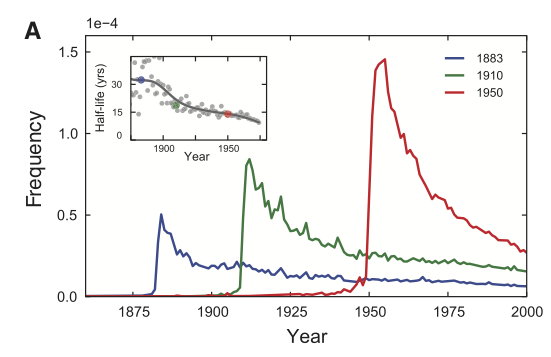
\includegraphics{michel_fig_3a.png}
\end{quote}

\hypertarget{part-a}{%
\section{Part A}\label{part-a}}

\begin{quote}
Get the raw data from the
\href{http://storage.googleapis.com/books/ngrams/books/datasetsv2.html}{Google
Books NGram Viewer website}. In particular, you should use version 2 of
the English language corpus, which was released on July 1, 2012.
Uncompressed, this file is 1.4GB.
\end{quote}

\hypertarget{get-and-clean-the-raw-data}{%
\subsection{Get and clean the raw
data}\label{get-and-clean-the-raw-data}}

Edit the \texttt{01\_download\_1grams.sh} file to download the
\texttt{googlebooks-eng-all-1gram-20120701-1.gz} file and the
\texttt{02\_filter\_1grams.sh} file to filter the original 1gram file to
only lines where the ngram matches a year (output to a file named
\texttt{year\_counts.tsv}).

Then edit the \texttt{03\_download\_totals.sh} file to down the
\texttt{googlebooks-eng-all-totalcounts-20120701.txt} and file and the
\texttt{04\_reformat\_totals.sh} file to reformat the total counts file
to a valid csv (output to a file named \texttt{total\_counts.csv}).

\hypertarget{load-the-cleaned-data}{%
\subsection{Load the cleaned data}\label{load-the-cleaned-data}}

Load in the \texttt{year\_counts.tsv} and \texttt{total\_counts.csv}
files. Use the \texttt{here()} function around the filename to keep
things portable.Give the columns of \texttt{year\_counts.tsv} the names
\texttt{term}, \texttt{year}, \texttt{volume}, and \texttt{book\_count}.
Give the columns of \texttt{total\_counts.csv} the names \texttt{year},
\texttt{total\_volume}, \texttt{page\_count}, and \texttt{book\_count}.
Note that column order in these files may not match the examples in the
documentation.

\begin{Shaded}
\begin{Highlighting}[]
\NormalTok{year_counts <-}\StringTok{ }\KeywordTok{read_tsv}\NormalTok{(}\StringTok{'year_count.tsv'}\NormalTok{, }\DataTypeTok{col_names =} \KeywordTok{c}\NormalTok{(}\StringTok{"term"}\NormalTok{, }\StringTok{"year"}\NormalTok{, }\StringTok{"volumn"}\NormalTok{, }\StringTok{"book_count"}\NormalTok{))}
\end{Highlighting}
\end{Shaded}

\begin{verbatim}
## Parsed with column specification:
## cols(
##   term = col_double(),
##   year = col_double(),
##   volumn = col_double(),
##   book_count = col_double()
## )
\end{verbatim}

\begin{Shaded}
\begin{Highlighting}[]
\NormalTok{total_counts <-}\StringTok{ }\KeywordTok{read_csv}\NormalTok{(}\StringTok{'total_count.csv'}\NormalTok{, }\DataTypeTok{col_names =} \KeywordTok{c}\NormalTok{(}\StringTok{"year"}\NormalTok{, }\StringTok{"total_volume"}\NormalTok{, }\StringTok{"page_count"}\NormalTok{, }\StringTok{"book_count"}\NormalTok{))}
\end{Highlighting}
\end{Shaded}

\begin{verbatim}
## Parsed with column specification:
## cols(
##   year = col_double(),
##   total_volume = col_double(),
##   page_count = col_double(),
##   book_count = col_double()
## )
\end{verbatim}

\begin{Shaded}
\begin{Highlighting}[]
\KeywordTok{head}\NormalTok{(year_counts)}
\end{Highlighting}
\end{Shaded}

\begin{verbatim}
## # A tibble: 6 x 4
##    term  year volumn book_count
##   <dbl> <dbl>  <dbl>      <dbl>
## 1  1817  1524     31          1
## 2  1817  1575     17          1
## 3  1817  1607      3          1
## 4  1817  1637      2          1
## 5  1817  1662      1          1
## 6  1817  1675      5          1
\end{verbatim}

\begin{Shaded}
\begin{Highlighting}[]
\KeywordTok{head}\NormalTok{(total_counts)}
\end{Highlighting}
\end{Shaded}

\begin{verbatim}
## # A tibble: 6 x 4
##    year total_volume page_count book_count
##   <dbl>        <dbl>      <dbl>      <dbl>
## 1  1505        32059        231          1
## 2  1507        49586        477          1
## 3  1515       289011       2197          1
## 4  1520        51783        223          1
## 5  1524       287177       1275          1
## 6  1525         3559         69          1
\end{verbatim}

\hypertarget{your-written-answer}{%
\subsection{Your written answer}\label{your-written-answer}}

Add a line below using Rmarkdown's inline syntax to print the total
number of lines in each dataframe you've created. Total number of lines
in year\_count.tsv is 53393

\hypertarget{part-b}{%
\section{Part B}\label{part-b}}

\begin{quote}
Recreate the main part of figure 3a of Michel et al.~(2011). To recreate
this figure, you will need two files: the one you downloaded in part (a)
and the ``total counts'' file, which you can use to convert the raw
counts into proportions. Note that the total counts file has a structure
that may make it a bit hard to read in. Does version 2 of the NGram data
produce similar results to those presented in Michel et al.~(2011),
which are based on version 1 data?
\end{quote}

\hypertarget{join-ngram-year-counts-and-totals}{%
\subsection{Join ngram year counts and
totals}\label{join-ngram-year-counts-and-totals}}

Join the raw year term counts with the total counts and divide to get a
proportion of mentions for each term normalized by the total counts for
each year.

\hypertarget{plot-the-main-figure-3a}{%
\subsection{Plot the main figure 3a}\label{plot-the-main-figure-3a}}

Plot the proportion of mentions for the terms ``1883'', ``1910'', and
``1950'' over time from 1850 to 2012, as in the main figure 3a of the
original paper. Use the \texttt{percent} function from the
\texttt{scales} package for a readable y axis. Each term should have a
different color, it's nice if these match the original paper but not
strictly necessary.

\hypertarget{your-written-answer-1}{%
\subsection{Your written answer}\label{your-written-answer-1}}

Write up your answer to Part B here.

\hypertarget{part-c}{%
\section{Part C}\label{part-c}}

\begin{quote}
Now check your graph against the graph created by the
\href{https://books.google.com/ngrams/}{NGram Viewer}.
\end{quote}

\hypertarget{compare-to-the-ngram-viewer}{%
\subsection{Compare to the NGram
Viewer}\label{compare-to-the-ngram-viewer}}

Go to the ngram viewer, enter the terms ``1883'', ``1910'', and ``1950''
and take a screenshot.

\hypertarget{your-written-answer-2}{%
\subsection{Your written answer}\label{your-written-answer-2}}

Add your screenshot for Part C below this line using the
\texttt{!{[}{]}(figure\_filename.png)} syntax and comment on
similarities / differences.

\hypertarget{part-d}{%
\section{Part D}\label{part-d}}

\begin{quote}
Recreate figure 3a (main figure), but change the y-axis to be the raw
mention count (not the rate of mentions).
\end{quote}

\hypertarget{plot-the-main-figure-3a-with-raw-counts}{%
\subsection{Plot the main figure 3a with raw
counts}\label{plot-the-main-figure-3a-with-raw-counts}}

Plot the raw counts for the terms ``1883'', ``1910'', and ``1950'' over
time from 1850 to 2012. Use the \texttt{comma} function from the
\texttt{scales} package for a readable y axis. The colors for each term
should match your last plot, and it's nice if these match the original
paper but not strictly necessary.

\hypertarget{part-e}{%
\section{Part E}\label{part-e}}

\begin{quote}
Does the difference between (b) and (d) lead you to reevaluate any of
the results of Michel et al.~(2011). Why or why not?
\end{quote}

As part of answering this question, make an additional plot.

\hypertarget{plot-the-totals}{%
\subsection{Plot the totals}\label{plot-the-totals}}

Plot the total counts for each year over time, from 1850 to 2012. Use
the \texttt{comma} function from the \texttt{scales} package for a
readable y axis. There should be only one line on this plot (not three).

\hypertarget{your-written-answer-3}{%
\subsection{Your written answer}\label{your-written-answer-3}}

Write up your answer to Part E here.

\hypertarget{part-f}{%
\section{Part F}\label{part-f}}

\begin{quote}
Now, using the proportion of mentions, replicate the inset of figure 3a.
That is, for each year between 1875 and 1975, calculate the half-life of
that year. The half-life is defined to be the number of years that pass
before the proportion of mentions reaches half its peak value. Note that
Michel et al.~(2011) do something more complicated to estimate the
half-life---see section III.6 of the Supporting Online Information---but
they claim that both approaches produce similar results. Does version 2
of the NGram data produce similar results to those presented in Michel
et al.~(2011), which are based on version 1 data? (Hint: Don't be
surprised if it doesn't.)
\end{quote}

\hypertarget{compute-peak-mentions}{%
\subsection{Compute peak mentions}\label{compute-peak-mentions}}

For each year term, find the year where its proportion of mentions peaks
(hits its highest value). Store this in an intermediate dataframe.

\hypertarget{compute-half-lifes}{%
\subsection{Compute half-lifes}\label{compute-half-lifes}}

Now, for each year term, find the minimum number of years it takes for
the proportion of mentions to decline from its peak value to half its
peak value. Store this in an intermediate data frame.

\hypertarget{plot-the-inset-of-figure-3a}{%
\subsection{Plot the inset of figure
3a}\label{plot-the-inset-of-figure-3a}}

Plot the half-life of each term over time from 1850 to 2012. Each point
should represent one year term, and add a line to show the trend using
\texttt{geom\_smooth()}.

\hypertarget{your-written-answer-4}{%
\subsection{Your written answer}\label{your-written-answer-4}}

Write up your answer to Part F here.

\hypertarget{part-g}{%
\section{Part G}\label{part-g}}

\begin{quote}
Were there any years that were outliers such as years that were
forgotten particularly quickly or particularly slowly? Briefly speculate
about possible reasons for that pattern and explain how you identified
the outliers.
\end{quote}

\hypertarget{your-written-answer-5}{%
\subsection{Your written answer}\label{your-written-answer-5}}

Write up your answer to Part G here. Include code that shows the years
with the smallest and largest half-lifes.

\hypertarget{makefile}{%
\section{Makefile}\label{makefile}}

Edit the \texttt{Makefile} in this directory to execute the full set of
scripts that download the data, clean it, and produce this report. This
must be turned in with your assignment such that running \texttt{make}
on the command line produces the final report as a pdf file.

\end{document}
